\documentclass[12pt]{article}

\usepackage[utf8]{inputenc}
\usepackage[francais]{babel}

\usepackage{amsmath}

\usepackage{caption}
\usepackage{subcaption}

\usepackage{tikz}
\usetikzlibrary{calc}

\definecolor{densitylow}{RGB}{255,220,220}
\definecolor{densitymedium}{RGB}{255,130,130}
\definecolor{densityhigh}{RGB}{255,50,50}

\usepackage[natbib=true,sorting=none,style=numeric,url=false,doi=false,isbn=false]{biblatex}
%\addbibresource{references}
\bibliography{references}

\begin{document}

\begin{titlepage}

  Stage de recherche

  {\Large \textsc{Coévolution du réseau viaire et du bâti}}

  \begin{flushright}
    \textit{Auteur :}\\
    Merwan {\scshape Achibet}\\[0.5cm]
    \textit{Encadrants :}\\
    Stefan {\scshape Balev}\\
    Antoine {\scshape Dutot}\\
    Damien {\scshape Olivier}
  \end{flushright}

  \vfill

  \begin{center}
    ILLUSTRATION
  \end{center}

  \vfill

  \begin{center}
    
\includegraphics[width=.25\linewidth]{images/logo-univ-le-havre.png}
    \qquad\qquad\qquad
    
\includegraphics[width=.25\linewidth]{images/logo-litis.png}
  \end{center}

  \begin{center}
    {\small Mars - Juin 2012}
  \end{center}

\end{titlepage}

\begin{center}
  {\scshape\textbf Keywords}
\end{center}

{Urban system, city morphogenesis, Voronoi diagram, cellular automaton.}

\begin{center}
  {\scshape\textbf Extended abstract}
\end{center}

Gathering issues of human, economic, geographic and political nature,
the city truly is a complex system. The increasing growth in
population produces urban systems like the world has never seen
before, of increasing size, increasing heterogeneity and increasing
complexity. Studying the relationships between its internal elements
is primordial to the understanding of its mechanics and to better
predict their developement. This work focuses on the relationship
between the pattern of human installations within the city --
characterized at the atomic level by a basic subdivision, the land lot
-- and its road network.

Systematic definitions of the city are many. Through the
anthropologist's eye it can be seen as a concentration of persons, the
economist will prefer to view it as a support for the exchange of
financial and physical assets and the urbanist as a functional entity
composed of flows and services. We choose to consider that the
evolution of a city is driven by its population, translated as a
measure of its density. This goes in hand with our focus as land lots
are inhabited by the same people using the surrounding roads to go
from one place to another and urbanistic decisions are motivated by a
need to optimize the city, streamlining transport means and avoiding
high contrasts in the urban fabric.

Study of the domain of urban simulations shows that available
scientific works can be classified in two different categories. For
visual rendering purposes, special effects in movies or video games,
methods have been proposed that generate visually satisfying cities
without regarding realism as an obligation. These are often based on
empirical observations and the main idea is to emulate the street
patterns found in any urban system. Scientific modeling, on the other
hand, prefers to focus on the inner qualities of a city, often by
studying a subset of those, to analyze its current state and
extrapolate its future. We orient our research with the latter in mind
but the former represents a non-negligible source of inspiration.

A reader browsing through the field litterature will often encounter
cellular automata. These structures, which applicability and potential
complexity has been proven over times, are fit for describing any kind
of space-related problem. Nevertheless, their rigorous formalism may
sometimes restrain realism and impact the validity of the model. For
example, a cellular automaton topology is, by definition, perfectly
regular and representing a city with a set of identical and aligned
cells seems like a coarse simplification. In the same way, the fact
that each cell has an identical neighborhood structure, the temporal
synchronism and the state discretization may be questionned. We take a
drastic step towards realism and embrace the spatial aspect of the
city by replacing the classic cellular automaton with a Voronoï
diagram following the same basic concepts. Each of its cell represents
a land lot and neighborhood relationships that are ruled by adjacency
determine its future state ; the regularity constraint is thus
relaxed. Voronoi edges delineate the Voronoi space of land lots and,
as such, are perfect supports for roads.

The different elements represented in our model (\textit{i. e. lots
  and roads}) are declined in two flavors. \textit{Potential} elements
have a ethereal status ; their spatial characteristics are known but
until they are definitely built, they have no direct effect on the
overall city and only represent an idea, a possible
outcome. \textit{Built} elements were potential elements that have
been constructed. They form the physical city. Concisely, the gist of
the model is to add potential elements to the city and, only later,
chose which ones will be built and which ones will be forgotten. The
road network expand to accomodate the growth in density and to support
anticipated land lots. This process has been divided into three
separate mechanisms.

The cellular part of the model lets the inner variables of the city
vary based on the Voronoi tesselation and a set of simple rules. Here,
only population density is considered and, as a result, the
characteristic gradual patterns found in most of the towns of the
world is reproduced.

Whereas the previous part of the model is ensuring vertical growth,
the horizontal component of the evolution of the city is handled by an
extensible method based on the use of vector fields. Each piece of
information that we want to consider is represented by a vector field
that will guide the placement of new lots. For example, a field
escaping from high density areas is used to ensure urban
sprawl. Another makes new lots move towards closest road such that
they remain snapped to the main road axes. All vector fields are then
summed up with varying coefficient. This general approach can model
any kind of guidance or constraint ; in particular obstacle avoidance
so that the city does not extends itself on forbidden areas like
lakes, beaches or protected forests.

The third and last mechanism chooses which of the potential elements
are to be permanently built. Potential roads are chosen with respect
to their contribution to the global network, by means of a network
flow evaluation. Potential land lots are chosen depending on their
position relative to the built roads and the date of their addition
into the potential domain.

RESULTATS/MESURES

MINI CONC

\newpage

\tableofcontents

\newpage

REMERCIEMENTS

\newpage

\section{Introduction}

LES VILLES GRANDISSENT

STATISTIQUES

POURQUOI ETUDIER CA ?

Il est nécéssaire d'étudier ces changements pour comprendre les
mécanismes sous-jacents à ce type de système et pour prévoir leur
évolution future. On se concentre ici sur l'évolution jointe de deux
ensembles majeurs du tissu urbain : le bâti et le viaire.

DETAILS

Ces deux aspects de la ville semblent aller de paire puisque le bâti
abrite les population tandis que le viaire leur permet de se
déplacer. Il est ainsi naturel d'utiliser la densité de population
comme force de guidage à l'évolution de la ville.

DETAILS

La première partie présente un état de l'art de la modélisation de
systèmes urbains et se concentre particulièrement sur les méthodes à
base d'automates cellulaires tout en adoptant un point de vue
historique pour justifier l'adoption de cette structure. Le modèle
conçu dans le cadre de ce stage de recherche est ensuite présenté en
seconde partie. La troisième section aborde des problématiques
pratiques rencontrées lors de l'implémentation dudit modèle. Enfin,
des mesures diverses sont employées pour tester et valider ce travail
dans la quatrième partie.

\section{\'Etat de l'art}

\subsection{Automates cellulaires et simulation urbaine}

La modélisation de systèmes complexes est longtemps uniquement passée
par l'usage de méthodes mathématiques; typiquement, des systèmes
d'équations différentielles. Ces techniques permettent de décrire des
lois d'évolution et d'observer, ainsi que de prédire par
extrapolation, le comportement de phénomènes du réel. Dans le cas de
modèles prenant en compte un vaste jeu de paramètres, cette approche
peut néanmoins se révéler délicate à employer. Plus intrinsèquement,
même si une telle modélisation est basée sur des observations ancrées
dans la réalité, il s'agit d'une représentation conceptuelle d'un
problème et aucune mimique des mécaniques sous-jacentes ne s'opère.

Historiquement, les prémices de l'informatique moderne et d'un tout
autre paradigme de modélisation sont à attribuer aux esprits du milieu
du vingtième siècle. Alan Turing introduit en 1936 la machine éponyme
qui, bien que purement théorique, possède un module de contrôle ainsi
qu'une mémoire et peut donc exécuter une infinité d'algorithmes. Cette
démarche se démarque de l'approche mathématique et semble plus
humaine; on ne résout pas un problème en utilisant des fonctions
associant une quantité à un résultat mais on agit véritablement sur
ses données. L'idée de base de Turing était d'ailleurs d'assimiler le
fonctionnement de sa machine au travail d'une personne remplissant les
cases d'un tableau infini.

Entraîné par cette mouvance procédurale et en réaction aux réseaux de
neurones de McCulloch et Pitts, John von Neumann et Stanislaw Ulam
joignent leurs travaux durant les années 40 pour concevoir l'automate
cellulaire : un système comprenant un ensemble d'automates à états
spatialement localisés (typiquement sous forme de grille) et
interconnectés en fonction de leur proximité. Les entrées de chaque
automate correspondent alors aux états des automates voisins et de
cette organisation se dégagent de fortes relations
d'interdépendance. Le jeu de la vie de Conway en est un exemple
classique. La simplicité de ses règles, mise en contraste avec la
variété des configurations engendrées, témoigne de la richesse des
automates cellulaires \cite{Gardner1970}.

Les automates cellulaires ont depuis été extensivement étudiés et sont
appliqués à l'étude de nombreux phénomènes biologiques, physiques et
sociaux \cite{Ganguly2003}. La motivation d'Ulam lors de leur
conception était d'ailleurs de modéliser la croissance de cristaux. On
peut aussi citer en exemple la simulation de la dynamique de fluides
\cite{Frisch1986} et de la croissance de tumeurs
\cite{Kansal2000}. Leur caractère spatial laisse supposer qu'ils sont
particulièrement adaptés aux applications géographiques, et dans le
cadre de notre problématique, urbaines. Ils ne fûrent paradoxalement
pas immédiatement exploités à cet effet et c'est seulement suite à un
article de Waldo Tobler, en 1975, que le rapprochement entre les
automates cellulaires et le domaine de la géographie apparaît
clairement \cite{Tobler1975}. Sont ensuite publiés des travaux majeurs
appliquant l'automate cellulaire à des problématiques géographiques
multi-échelles telles que l'évolution d'épidémies \cite{Fu2003} et la
ségrégation de population \cite{Schelling1969} (voir figure
\ref{fig:schelling}).

\begin{figure}
  \centering
  
\includegraphics[width=.6\linewidth]{images/schelling.png}
  \caption{Configuration produite par le modèle de Schelling. Chacune
    des deux couleurs représente une population différente. La
    conclusion de ces travaux est qu'un faible degré d'animosité entre
    deux populations suffit à les séparer de manière évidente.}
  \label{fig:schelling}
\end{figure}

Une idée très exploitée dans ce domaine est d'associer un potentiel de
transition à chaque cellule et ce, vers tous les états qu'elles
peuvent adopter. Dans les modèles déterministes, la transition vers
l'état à plus haut potentiel est appliquée tandis que dans les modèles
stochastiques, un tirage aléatoire biaisé est préféré. Le potentiel
d'une cellule à passer à un nouvel état est déterminé en fonction de
paramètres propres au modèle. Peuvent être pris en compte l'élévation
du terrain, la densité de population, la proximité d'axes routiers, la
proximité de centres urbains, l'âge des parcelle, leur valeur; en
fait, toute combinaison d'attributs relatifs à un réseau urbain. Par
exemple, dans une simulation représentant les différents types
d'usage, le passage d'une cellule à l'état \textit{résidentiel}
pourrait dépendre de la proximité des commerces et des routes et de
l'éloignement des zones industrielles. Bien sûr, un nombre élevé de
paramètres à prendre en compte requiert un couplage fin et l'impact de
chaque variable peut être pondéré. Puisque les variations
individuelles de paramètres n'émergent pas de manière transparente à
la surface de la simulation, les modèles urbains basés sur des
automates cellulaires doivent être finement calibrés et leur réalisme
est un défi en soi. Pour contourner ce problème, Yeh et Li prônent
l'usage d'un réseau de neurones pour pondérer chaque paramètre à
partir de l'analyse de données cartographiques historiques
\cite{Yeh2002}.

Il est important de noter que la simplicité du formalisme enveloppant
un automate cellulaire strict s'oppose à la qualité de la simulation,
notamment dans le cadre de modèles spécifiques
\cite{Torrens2001}. Dans ce cas, une prise de liberté quant aux
formalisme originel est autorisée, voire nécessaire, pour obtenir des
résultats satisfaisants \cite{White1998}.

La première limite que le formalisme cellulaire de base impose est la
discrétisation des états que chaque cellule peut adopter. Même si
cette caractéristique fait partie intégrante des particularités qui
confèrent aux automates cellulaires leur simplicité d'usage et
d'analyse, la description de quantités pouvant arborer un éventail
infini de valeurs est alors impossible. Plus concrètement, il est aisé
de catégoriser les cellules d'un espace selon le fait, par exemple,
qu'elles contiennent des installations humaines ou non (état booléen)
\cite{Benguigui2004,Cornu2008} ou de façon plus sophistiquée, en
fonction de leur type d'usage (\textit{résidentiel},
\textit{commercial} et \textit{industriel} \cite{Lechner} et plus
\cite{Dubos-Paillard2003}). Représenter des quantités réelles et des
variations continues est moins aisé. Pour symboliser plus finement la
densité au c\oe ur d'un ensemble urbain, Semboloni utilise par exemple
un automate cellulaire de dimension trois dans lequel plus une pile de
cellules actives est haute et plus la zone représentée est peuplée
\cite{Semboloni2000}. Plus généralement, il est accepté de représenter
l'état d'une cellule par un vecteur contenant des valeurs réelles; des
règles de transitions adaptées et mesurées sont alors à mettre en
place.

L'homogénéité d'un automate cellulaire fait partie intégrante de sa
définition originelle : en mettant de côté l'état qu'elles adoptent,
toutes les cellules sont identiques en forme et en structure de
voisinage. Dans le cadre de notre problématique, cette approche est
limitante car, dans une ville, les parcelles ne sont que rarement
identiques et alignées. Similairement, la notion de voisinage est
clairement à redéfinir. Pour des problèmes classiques, les voisinages
de von Neumann et de Moore sont régulièrement utilisés mais la
relation par contiguité qu'ils décrivent ne convient pas à la
représentation des liens de dépendance à plus grande échelle se
développant dans un système urbain. Le positionnement d'un bâtiment
résidentiel dans une ville se base évidemment sur le voisinage direct
des zones envisagées (on préfère construire une maison dans un
quartier résidentiel) mais il faut aussi prendre en compte les
alentours plus distants (la centrale thermique se trouvant à 500
mètres du site peut poser problème). Une solution possible est
d'étendre les aires des voisinages de von Neumann et de Moore tout en
conservant leur forme caractéristique. La symétrie évidente se
dégageant de telles simplifications va à l'encontre des relations
prenant place au sein d'une ville dont les zones ne sont que très
rarement parfaitement disposées. O'Sullivan a choisi de relaxer cette
contrainte de partionnement spatial régulier pour faire un pas dans la
direction du réalisme \cite{O'Sullivan2000,O'Sullivan2001} :
conventionnellement, une cellule d'automate correspond à un
sous-espace urbain ou bien une parcelle cadastrale mais dans chacun de
ces cas le modèle se base évidemment sur une simplification grossière
de l'espace étudié. Il décide donc de donner à chaque cellule les
mêmes qualités topologiques que les parcelles qu'elles représentent :
même formes, même dimensions, mêmes coordonnées. Une variété de
relations de voisinage sont alors envisageables (par voisinage au sens
urbain, par distance dans un rayon d'influence, par critère de
visibilité). L'éloignement du formalisme cellulaire est drastique car
la structure perd de son homogénéité (chaque cellule est différente),
la couverture de l'espace n'est plus complète (des vides entre les
cellules apparaissent) et le voisinage diffère lui aussi mais chacun
de ces changements ???.

\begin{figure}
  \centering
  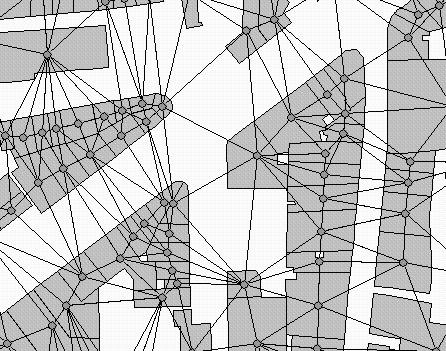
\includegraphics[width=.7\linewidth]{images/gca.png}
  \caption{Hoxton, un quartier de Londres, modélisé par l'automate
    cellulaire graphe de David O'Sullivan \cite{O'Sullivan2000}.}
  \label{fig:sullivan}
\end{figure}

\begin{figure}
  \begin{subfigure}[b]{.5\linewidth}
    \centering
    \begin{tikzpicture}
  \draw[step=1,gray] (0,0) grid (3,3);

  \node at (0.5,0.5) {G};
  \node at (1.5,0.5) {H};
  \node at (2.5,0.5) {I};
  \node at (0.5,1.5) {D};
  \node at (1.5,1.5) {E};
  \node at (2.5,1.5) {F};
  \node at (0.5,2.5) {A};
  \node at (1.5,2.5) {B};
  \node at (2.5,2.5) {C};
\end{tikzpicture}

    \caption{Automate cellulaire classique.}
  \end{subfigure}
  \begin{subfigure}[b]{.5\linewidth}
    \centering
    \begin{tikzpicture}
  \draw (0.5,0.5) node[circle,draw] (g) {G};
  \draw (1.5,0.5) node[circle,draw] (h) {H};
  \draw (2.5,0.5) node[circle,draw] (i) {I};
  \draw (0.5,1.5) node[circle,draw] (d) {D};
  \draw (1.5,1.5) node[circle,draw] (e) {E};
  \draw (2.5,1.5) node[circle,draw] (f) {F};
  \draw (0.5,2.5) node[circle,draw] (a) {A};
  \draw (1.5,2.5) node[circle,draw] (b) {B};
  \draw (2.5,2.5) node[circle,draw] (c) {C};

  \draw (a) -- (b);
  \draw (a) -- (e);
  \draw (a) -- (d);
  \draw (b) -- (c);
  \draw (b) -- (f);
  \draw (b) -- (e);
  \draw (b) -- (d);
  \draw (b) -- (f);
  \draw (c) -- (f);
  \draw (d) -- (e);
  \draw (d) -- (h);
  \draw (d) -- (g);
  \draw (e) -- (c);
  \draw (e) -- (f);
  \draw (e) -- (i);
  \draw (e) -- (h);
  \draw (e) -- (g);
  \draw (f) -- (i);
  \draw (f) -- (h);
  \draw (g) -- (h);
  \draw (h) -- (i);
\end{tikzpicture}

    \caption{Automate cellulaire graphe.}
  \end{subfigure}
\end{figure}

Une prise de liberté quant à l'aspect temporel est aussi
envisageable. Un automate cellulaire strict est synchrone,
\textit{i. e.} les changements d'état de toutes les cellules
s'effectuent simultanément. Si le choix était fait de mettre à jour
chaque état de façon asynchrone, le comportement de l'automate en
serait lourdement modifié. Par exemple, les qualités auto-réplicatives
de certaines entités du jeu de la vie ne seraient pas garanties. Il
est pourtant légitime de se questionner sur la validité d'un tel choix
dans une simulation urbaine, premièrement parce qu'une ville est un
système complexe et désordonné, deuxièmement parce les processus qui
s'y déroulent sont réglés sur différentes échelles temporelles.

Bien que les automates cellulaires soient couramment utilisés pour
simuler le traffic routier (dans leur version 1D CITATION ou 2D
\cite{Queloz1996}), ils s'accordent peu avec la construction même d'un
réseau viaire. Dans les simulations cellulaires urbaines, le
positionnement des routes a un impact sur le développement des
cellules puisque le viaire \textit{attire} le bâti mais le réseau est
souvent fourni en entrée et reste fixe. Nous sommes amener à nous
interroger sur la capacité des automates cellulaires à modéliser le
développement routier. Les relations de proximité les caractérisant
sont-elles adaptées à la construction de structures dont l'échelle est
celle de la ville et non plus celle de la parcelle ? REPONSE

\subsection{Approches alternatives}

Les automates cellulaires ne sont pas l'unique moyen de modéliser la
croissance urbaine. Plusieurs simulations existantes sont des systèmes
multi-agent \cite{Lechner2003,Lechner2004}. Dans ces cas, un agent est
assimilé à un promoteur immobilier et peut acheter des terres, les
vendre, les développer ou changer leur type. Les actions qu'il
entreprend sont évaluées en fonction de l'impact sur la ville
(changement de la valeur immobilière, avis de la population) et des
réglementations locales afin d'éviter toute configuration illégale.
Pour la construction du réseau routier, une solution est de mettre en
place, en plus des agents promoteurs, deux types d'agents
traceurs. Les \textit{extenders} parcourent toute la surface du
terrain à la recherche de bâtiments isolés puis tracent une route
jusqu'au réseau urbain. Les \textit{connectors} se déplacent
uniquement sur le réseau viaire et y raccordent les bâtiments non
connectés se trouvant dans leur rayon de détection
\cite{Lechner2003}. Ce genre d'approche quant à la coévolution entre
routes et bâti introduit un défaut : le réseau viaire est construit à
partir du bâti et des bâtiments peuvent rester isolés. PLUS?

D'autres solutions s'éloignant des systèmes complexes et penchant du
côté de la génération procédurale de contenu existent. Souvent, le
domaine d'application de telles méthodes est l'infographie, le cinéma
et le jeu vidéo et l'objectif est alors de construire de manière
automatique une ville visuellement réaliste sans se soucier de son
caractère fonctionnel. Usuellement, l'organisation parcellaire dépend
entièrement du réseau routier car la première étape est souvent de
générer un réseau viaire complet puis de placer le bâti en subdivisant
récursivement les niches vides formées par les voies. Dans Citygen
\cite{Kelly2006b}, un point $p$ de l'espace est aléatoirement choisi
puis on calcule un ensemble de plusieurs routes raccordant $p$ au
réseau routier existant en faisant varier leur déviation angulaire et
un paramètre de bruit; la route finale est celle pour laquelle la
variation d'altitude est la plus faible. CityEngine \cite{Parish2001}
utilise un L-System dont les règles permettent de reproduire les
différents motifs quadrillés, radiaux et organiques que l'on retrouve
dans une ville. La nature récursive des L-Systems permet à ces motifs
de se combiner et d'apparaître à différents niveaux de profondeur
(voir figure \ref{fig:cityengine}). Dans une autre simulation, le
tracé des routes suit les \textit{hyperstreamlines} \cite{Chen2008}
formées par un champ de vecteurs. Ce champ est calculé par combinaison
de plusieurs autres champs de vecteurs, chacun représentant des
contraintes directionnelles particulières telles que les zones
interdites (eau, espaces verts), l'altitude et la densité de
population. Ces techniques sont intrinsèquement géométriques, et comme
précisé plus haut, le résultat est purement visuel, mais elles
représentent une source d'inspiration à ne pas négliger.

\begin{figure}
  \centering
  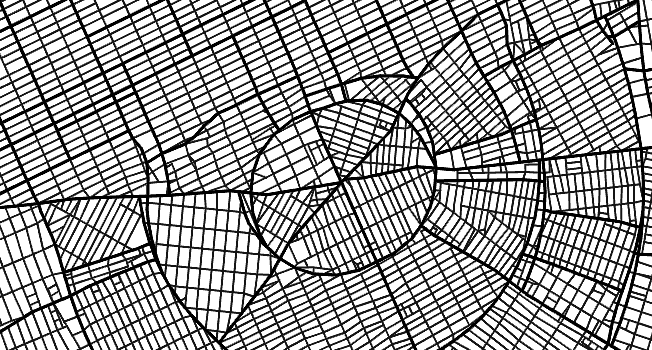
\includegraphics[width=.8\linewidth]{images/cityengine.png}
  \caption{CityEngine mélange des motifs urbains extraits de cartes de
    Paris et de New York \cite{Parish2001}.}
  \label{fig:cityengine}
\end{figure}

L'un des rares modèles gérant à la fois l'évolution du réseau viaire
et du bâti est présenté par Weber \cite{Weber2009} et n'emploie pas
d'automate cellulaire. Le principe est le suivant : à chaque
agrandissement du réseau urbain, on crée plusieurs routes virtuelles
en suivant des règles géométriques précises (allongement des voies
existantes, limitation du degré des carrefours à 4, l'angle entre
chaque rue tend vers 90 degrés). Parmi les $n$ routes générées, une
seule sera construite. Pour la choisir, le traffic sur ces nouvelles
routes est simulé par des agents piétons et véhicules et l'on
identifie celle qui sera la plus bénéfique au réseau.

\section{Le modèle}

\subsection{Structure}

Les automates cellulaires sont des structures versatiles et puissantes
dont le formalisme originel impose néanmoins quelques limitations;
l'une des principales étant, à nos yeux, un maillage régulier et
statique. Pour répondre à notre problématique, il est nécessaire
d'employer une structure respectant les critères suivants :

\begin{enumerate}
\item{Elle doit partitionner l'espace, possiblement de façon
  irrégulière;}
\item{Des relations de voisinages pourront être déduites de sa
  topologie;}
\item{Elle doit pouvoir représenter à la fois la parcellisation du
  territoire et le réseau routier.}
\end{enumerate}

Le diagramme de Voronoï est un candidat idéal. Sa constitution est
intrinsèquement spatiale puisqu'il s'agit d'un partionnement axé
autour de points spéciaux, les générateurs, chacun possédant une
cellule contenant tous les points plus proches de ce générateur que de
tout autre. Autrement dit, la distance séparant un point $p$ placé
dans une cellule de Voronoï et le générateur de cette même cellule est
inférieure à la distance séparant $p$ de tous les autres générateurs
\cite{Edwards1993}. La figure \ref{fig:voronoi} fournit un exemple de
diagramme de Voronoï et on remarque que, naturellement, deux
générateurs voisins sont équidistants de l'arête les séparant et le
segment les reliant y est perpendiculaire. DEFINITION PLUS FORMELLE ?

\begin{figure}[h]
  \centering
  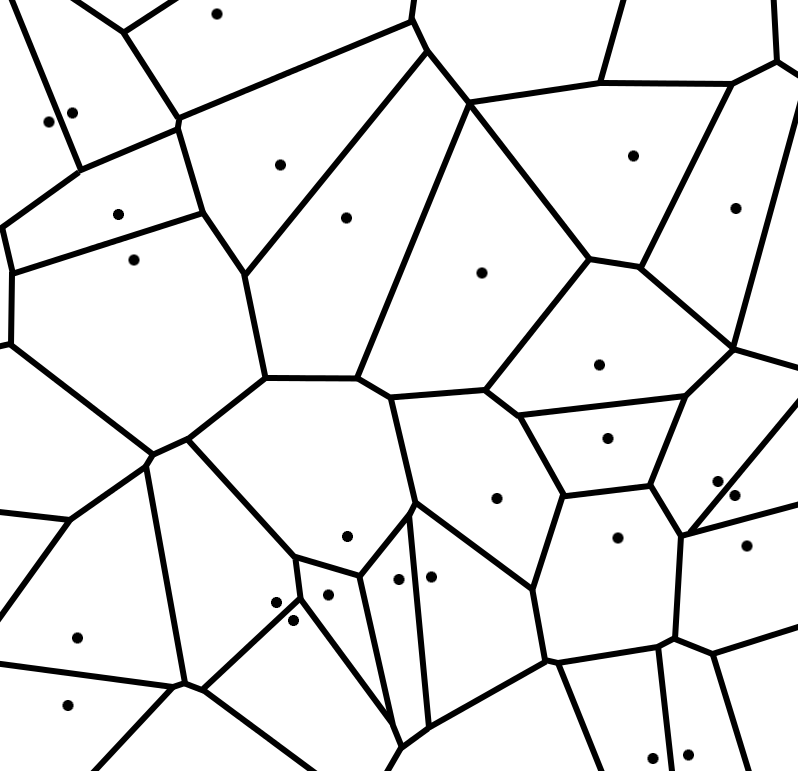
\includegraphics[width=0.5\linewidth]{images/voronoi.png}
  \caption{Un diagramme de Voronoï. Chaque point noir est un générateur.}
  \label{fig:voronoi}
\end{figure}

Les diagrammes de Voronoï trouvent de nombreuses applications en
science. En robotique, les obstacles présents dans un environnement
peuvent être assimilés à des générateurs et un robot cherchant à
maximiser leur évitement préférera longer les frontières des cellules
(les arêtes de Voronoï) \cite{Garrido2006}. En sociologie
géographique, ils permettent d'opposer les zones d'influence de
différents éléments urbains et répondent à des questions telles que :
quel magasin un piéton sera-t-il plus susceptible de visiter selon la
zone dans laquelle il se trouve ? Leur utilisation pour l'étude de
l'épidémie de choléra londonienne en 1854 à permis de vérifier le lien
entre fontaines publiques infectées (les générateurs) et zones
souffrant d'un fort taux de mortalité (les cellules)
\cite{Thomas2010}.

Comme som homonymie le laisse présager, la cellule de Voronoï remplace
la cellule carrée de l'automate cellulaire. On remarque qu'une grille
régulière, comme celles présentes dans les automates cellulaires
classiques correspond à un diagramme de Voronoï dans laquelle les
générateurs sont alignés et régulièrement disposés. Une tesselation de
Voronoï peut être considérée comme une généralisation de la structure
grillagée ; notre première contrainte est satisfaite.

À l'échelle de ce modèle, chaque cellule représente une parcelle
cadastrale et on utilise comme générateur le centre de son
empreinte. Le diagramme permet d'identifier les parcelles voisines
comme étant celles partageant une arête de Voronoï. Un graphe de
voisinage est ainsi construit, et adopte la forme duale du diagramme
de Voronoï : la triangulation de Delaunay. Ce premier graphe décrit le
réseau de voisinage mettant en relation les parcelles en contact à
partir du diagramme et satisfait donc la seconde contrainte.

Cette structure permet de décrire un canevas urbain de base dans
lequel l'espace d'influence de chaque parcelle est décrit mais la
composante routière reste encore absente du modèle. Chaque arête de
Voronoï indique un espace entre deux parcelles et est donc susceptible
d'accueillir une route. Dans une véritable ville, chaque parcelle
n'est pas encerclée de voies et l'un des objectifs de la simulation
est de déterminer quelles arêtes accueilleront des routes et
lesquelles resteront vides. Le diagramme de Voronoï suffit bien à
représenter à la fois les éléments du viaire et du bâti et notre
dernière contrainte est comblée.

En réalité, dans ce modèle la ville est représentée par deux graphes
et le diagramme de Voronoï est uniquement employé en tant que point de
départ. Le premier, le graphe du bâti, a pour n\oe ud les centres des
parcelles alors que ses arêtes symbolisent les relations de
voisinage. Le second, le graphe viaire, a des arêtes représentant les
routes et des n\oe uds carrefour joignant plusieurs voies. Les
structures des graphe viaire et bâti sont donc entièrement fondées sur
le diagramme de Voronoï puisqu'il s'agit, respectivement, de
l'ensemble des arêtes et sommets de Voronoï et de sa triangulation de
Delaunay. REFORMULER

Il est essentiel de dissocier le polygone convexe qu'est la cellule de
Voronoï associée à une parcelle et la véritable empreinte cadastrale
de cette dernière. Une cellule représente l'influence d'une parcelle
dans l'espace urbain et possède comme seul point commun avec
l'empreinte son centre puisqu'il s'agit du générateur de la
cellule. Similairement, une arête peut indiquer qu'une voie passe
entre deux parcelles sans pour autant fournir ses coordonnées ou sa
courbure. Si l'on souhaite, dans un but infographique, générer une
image de notre ville à partir de ce modèle, un travail
d'interprétation est nécessaire et n'a pas été traîté à l'occasion de
ce projet. Un exemple est visible sur la figure \ref{fig:interp}.

\begin{figure}[h]

  \centering
  \subcaptionbox{}[0.9\linewidth][c]{
    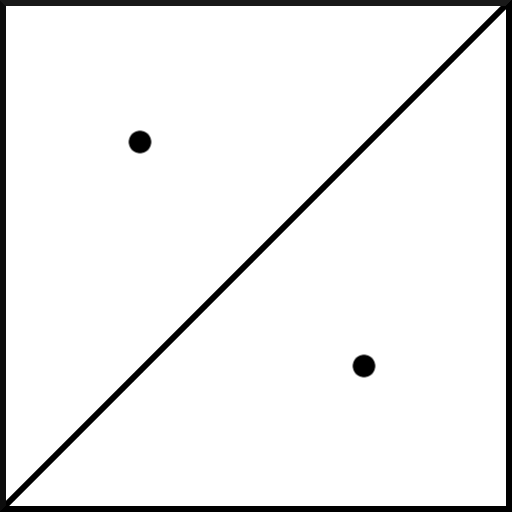
\includegraphics[width=.3\linewidth]{images/voronoi-interp0.png}
  }

  \subcaptionbox{}[.3\linewidth][c]{
    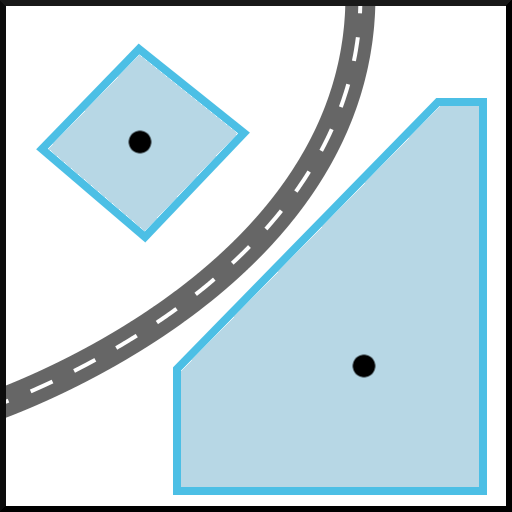
\includegraphics[width=.3\linewidth]{images/voronoi-interp1.png}
  }
  \subcaptionbox{}[.3\linewidth][c]{
    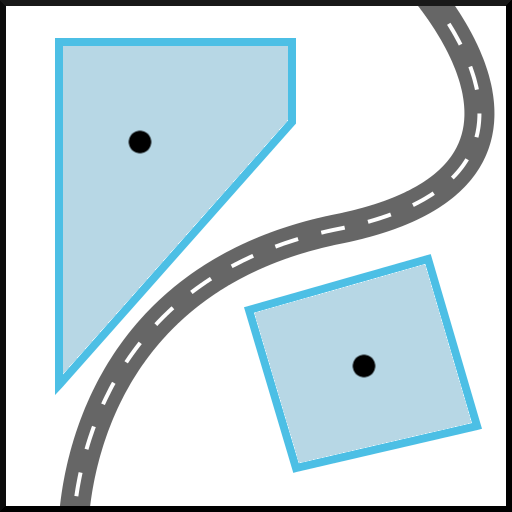
\includegraphics[width=.3\linewidth]{images/voronoi-interp2.png}
  }
  \subcaptionbox{}[.3\linewidth][c]{
    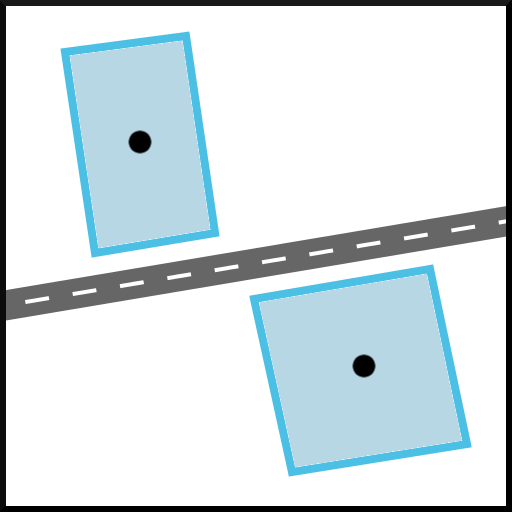
\includegraphics[width=.3\linewidth]{images/voronoi-interp3.png}
  }

  \caption{Un diagramme de Voronoï trivial et trois interprétations possibles.}
  \label{fig:interp}
\end{figure}

\subsection{Potentialité}

Via le terme \textit{potentialité}, on souhaite exprimer l'opposition
entre deux types d'éléments : les \textit{potentiels} et les
\textit{construits}.

Un élément \textit{construit} est une parcelle ou une voie dont
l'existence physique est avérée. Il existe \textit{en dur} et affecte
ses alentours. L'ensemble des éléments construit forme la ville (voir
figure \ref{fig:construit}).

\begin{figure}
  \centering
  IMAGE
  \caption{Les éléments construits forment la ville.}
  \label{fig:construit}
\end{figure}

Un élément \textit{potentiel} peut être assimilé à une idée germant
dans l'esprit de l'urbaniste ; à une possibilité envisagée et
représentée de manière intangible. Un élément potentiel est par la
suite soit construit, soit ignoré et oublié. Il sert de prévision à
court-terme quant à l'avenir de la ville et guide sa morphogénèse. La
figure \ref{fig:potentiel} reprend la micro-ville de la figure
\ref{fig:construit} et laisse apparaître voies et parcelles
potentielles.

\begin{figure}
  \centering
  IMAGE A FAIRE
  \caption{Les éléments potentiels guident la croissance
    de la ville.}
  \label{fig:potentiel}
\end{figure}

Un élément potentiel, n'étant pas actif au sein de la ville et
appartenant uniquement au domaine du prévisionnel, n'a pas d'influence
sur les éléments construits. Par contre, la construction de nouveaux
éléments peut en dépendre \textit{e.g.} une route peut être construite
en conséquence à cette prévision, comme attirée par cette portentielle
future installation. Cette dualité dont les relations d'influence sont
clairement unidirectionnelles est inspirée du cycle réel
d'urbanisation que l'on pourrait grossièrement décomposer en ces
quelques étapes :

\begin{enumerate}
\item{Un urbaniste prévoit une nouvelle installation en bordure de
  ville}
\item{Cette prévision attire la route}
\item{La nouvelle route et l'installation potentielle attirent
  d'autres installations potentielles}
\end{enumerate}
REFORMULER

L'essence du modèle est de placer des éléments potentiels en fonctions
de qualités internes au système puis de choisir lesquels véritablement
construire. Ce travail a été décomposé en trois mécanismes
distincts. ETOFFER

\subsection{Mécanismes}

\subsubsection{Automate cellulaire graphe}

La dynamique de croissance urbaine est décomposable sur deux axes. La
croissance horizontale décrit l'expansion spatiale de la ville dont
l'enveloppe grandit pour occuper plus de territoire tandis que la
croissance verticale correspond à l'augmentation des densités au sein
de la ville, souvent à partir d'un ou de plusieurs centres. Le
mécanisme cellulaire présenté ci-après émule la croissance verticale
et les variations de densité internes au système.

La densité de population est la quantité principale guidant
l'évolution de ce modèle. Même si le mécanisme proposé reste
trivialement simple, il guide les autres mécanismes du modèle : le
placement de nouvelles parcelles et le choix des routes à
construire. La ville évolue, de nouveaux bâtiments apparaissent,
d'autres sont rasés, les quartiers changent et le modèle doit être
capable de simuler ces changements. C'est bien sûr avec le principe
des automates cellulaires en tête que nous allons gérer cette
dynamique.

On discrétise la densité sur trois paliers : \textit{faible} ($f$),
\textit{moyenne} ($m$) et \textit{élevée} ($e$). L'état d'une parcelle
dépend des états de ses voisines. La matrice $A$ décrit des
coefficients d'affinité mettant en relation les différentes
densités.

\begin{equation}
A =
\bordermatrix{
    & f & m & e \cr
  f & 1 & 0.01 & 0 \cr
  m & 0.001 & 1.5 & 0.01 \cr
  e & 0 & 0.01 & 1.6
}
\end{equation}

Une valeur haute en $A_{ee}$ signifie par exemple que si une cellule a
de nombreux voisins de densité \textit{élevée} alors elle a une grande
probabilité de devenir elle-même \textit{élevée}. L'équation
\ref{eq:transition} permet de formaliser ce principe et fournit un
score $T$ pour chaque état d'arrivée possible. $C$ correspond à la
cellule dont l'on étudie les possibilités et $V_k(C)$ correspond au
nombre de voisins de $C$ ayant l'état $k$.

\begin{equation}
T_i(C) = \sum_{k \in \{f,m,e\}} V_k(C) E_{ik}
\label{eq:transition}
\end{equation}

Finalement et pour obtenir la
véritable probabilité de passage d'un état à un autre, on normalise
chaque score de transition et une roue de la fortune biaisée se charge
du choix.

\begin{equation}
P_i(C) = \frac{T_i(C)}{\sum_{k \in \{f,m,e\}} T_k(C)}
\label{eq:normalisation}
\end{equation}

Imaginons un exemple trivial pour illustrer ce processus. On considère
l'état que prendra la cellule $C$, au centre du quadrillage de la
figure \ref{fig:ca-example}. On commence par calculer les scores de
transition en fonction du voisinage de $C$.

\begin{figure}[h]
  \centering
  \begin{tikzpicture}

  \fill[densitylow] (0,0) rectangle (1,1);
  \fill[densitymedium] (1,0) rectangle (2,1);
  \fill[densityhigh] (2,0) rectangle (3,1);
  \fill[densitymedium] (0,1) rectangle (1,2);
  \fill[densitymedium] (1,1) rectangle (2,2);
  \fill[densityhigh] (2,1) rectangle (3,2);
  \fill[densitymedium] (0,2) rectangle (1,3);
  \fill[densityhigh] (1,2) rectangle (2,3);
  \fill[densityhigh] (2,2) rectangle (3,3);

  \draw[step=1,black] (0,0) grid (3,3);

  \draw[black,line width=2] (1,1) rectangle (2,2);
\end{tikzpicture}

  \caption{On cherche à calculer les probabilités transitionnelles
    pour la cellule centrale, $C$.}
  \label{fig:ca-example}
\end{figure}

\begin{align*}
T_f(C) &= V_f(C) A_{ff} + V_m(C) A_{fm} + V_e(C) A_{fe} \\
       &= 1 \times 1 + 3 \times 0.01 + 4 \times 0 \\
       &= 1.03
\end{align*}

\begin{align*}
T_m(C) &= V_f(C) A_{mf} + V_m(C) A_{mm} + V_e(C) A_{me} \\
       &= 1 \times 0.001 + 3 \times 1.5 + 4 \times 0.01 \\
       &= 4.541
\end{align*}

\begin{align*}
T_e(C) &= V_f(C) A_{ef} + V_m(C) A_{em} + V_e(C) A_{ee} \\
       &= 1 \times 0 + 3 \times 0.01 + 4 \times 1.6 \\
       &= 6.7
\end{align*}

On normalise ensuite les scores afin de sélectionner aléatoirement --
mais de façon biaisée -- le prochain état de $C$. Ici, on observe que
la cellule a de fortes chances de passer à la densité \textit{élevée}.

\begin{equation*}
P_f(C) = \frac{T_f(C)}{\sum_{k \in \{f,m,e\}} T_k(C)} = \frac{1.03}{1.03 + 4.541 + 6.7} = 0.084
\end{equation*}

\begin{equation*}
P_f(C) = \frac{T_f(C)}{\sum_{k \in \{f,m,e\}} T_k(C)} = \frac{1.03}{1.03 + 4.541 + 6.7} = 0.37
\end{equation*}

\begin{equation*}
P_f(C) = \frac{T_f(C)}{\sum_{k \in \{f,m,e\}} T_k(C)} = \frac{1.03}{1.03 + 4.541 + 6.7} = 0.546
\end{equation*}

\begin{figure}[h]
  \centering
  \begin{tikzpicture}[rotate=-90,xscale=-1]

  \draw[black,fill=densitylow] (0,0) -- (0:2) arc (0:33:2) -- cycle;
  \draw[black,fill=densitymedium] (0,0) -- (33:2) arc (33:166:2) -- cycle;
  \draw[black,fill=densityhigh] (0,0) -- (166:2) arc (166:360:2) -- cycle;

\end{tikzpicture}

  \caption{LEGENDE}
\end{figure}
VRAIMENT UTILE ?

Ce processus d'attraction évoque le modèle de ségrégation de Schelling
à la différence qu'ici trois types de \textit{population}
interagissent et qu'il n'y a pas de contrainte de déménagement (dans
son modèle, si une cellule passe de $A$ à $B$ alors une autre doit
passer de $B$ à $A$ afin de conserver les mêmes quantités de chaque
type). Ainsi un dégradé discret de densité apparaît comme dans une
ville réelle.

On commence par appliquer cette règle a un automate cellulaire
classique (voir figure \ref{fig:ac}).

\begin{figure}[h]
  \centering
  \subcaptionbox{$t = 0$}[.3\linewidth][c]{
    
\includegraphics[width=.3\linewidth]{images/ca_0.png}
  }
  \subcaptionbox{$t = 25$}[.3\linewidth][c]{
    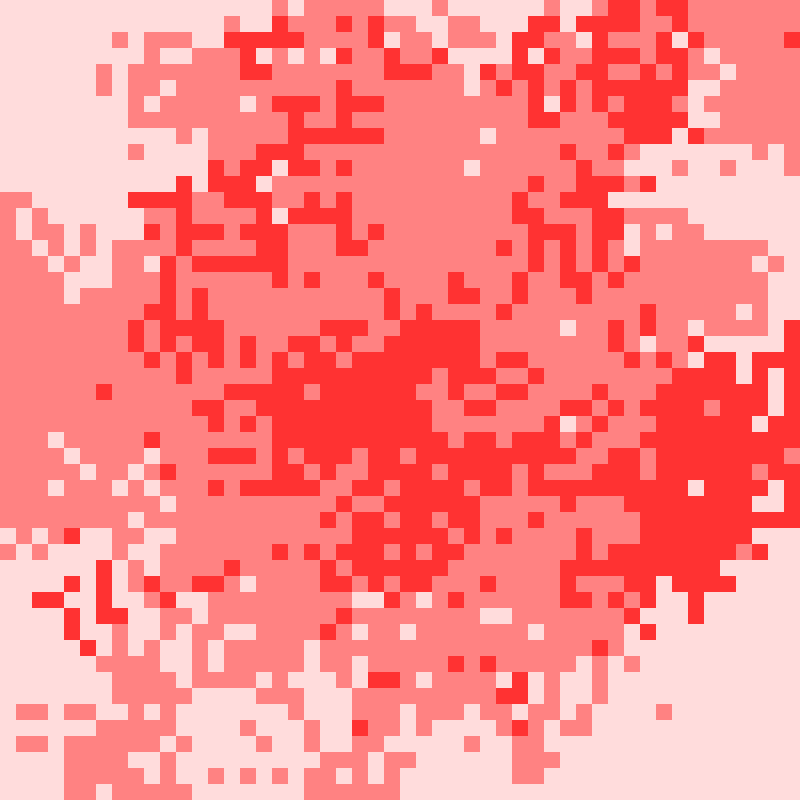
\includegraphics[width=.3\linewidth]{images/ca_25.png}
  }

  \subcaptionbox{$t = 50$}[.3\linewidth][c]{
    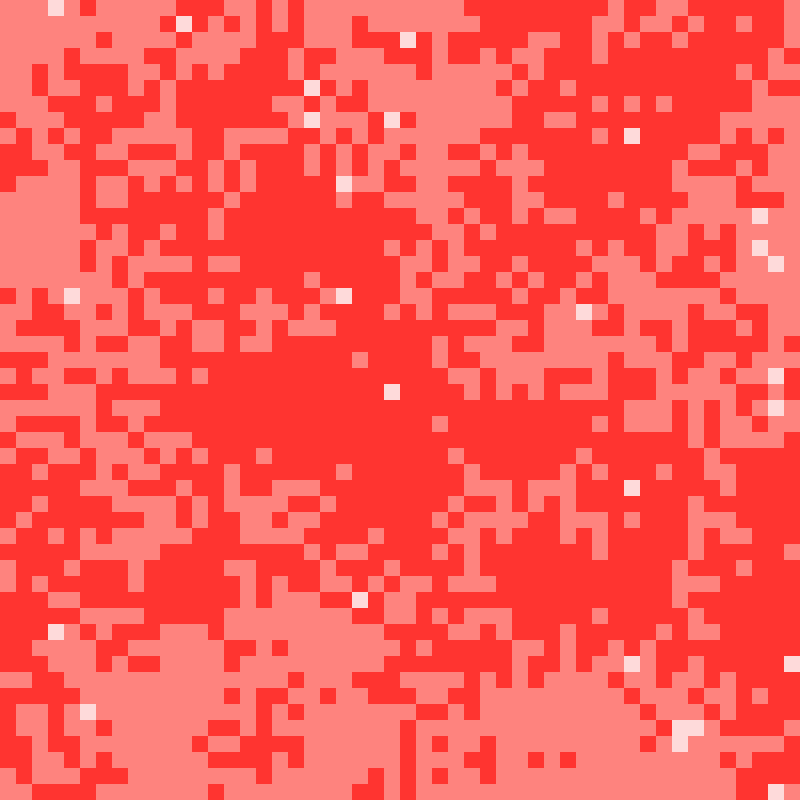
\includegraphics[width=.3\linewidth]{images/ca_50.png}
  }
  \subcaptionbox{$t = 100$}[.3\linewidth][c]{
    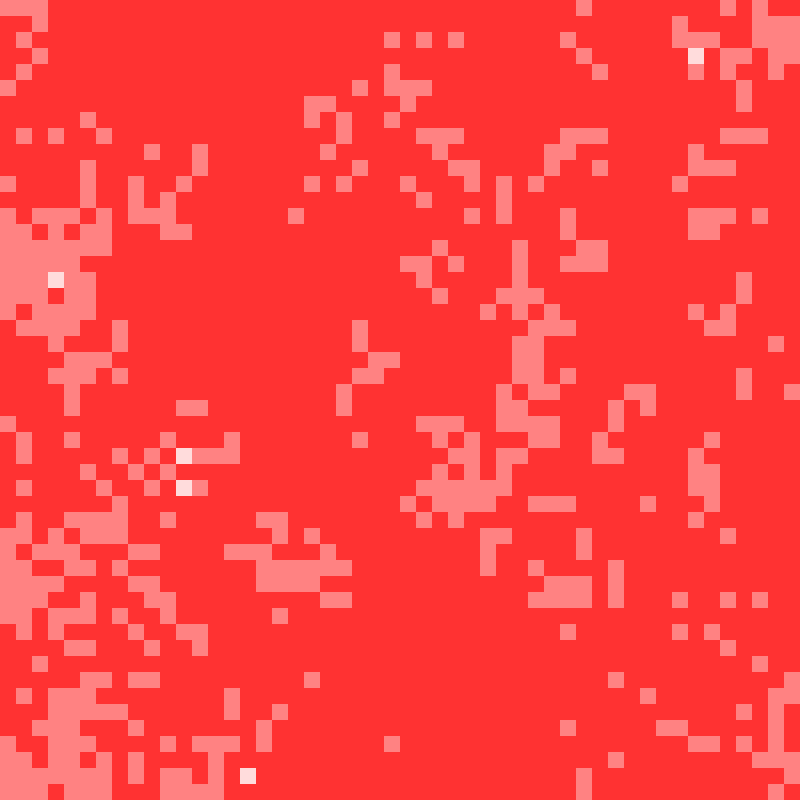
\includegraphics[width=.3\linewidth]{images/ca_100.png}
  }
  \caption{Quatre configurations de l'automate cellulaire. On y
    retrouve peu de similarités et les changements sont très rapides.}
  \label{fig:ac}
\end{figure}

On remarque deux problèmes. Premièrement, l'automate est très
rapidement métamorphosé. \`A l'itération 25, la disposition de départ
n'est déjà plus discernable. Hors, la granularité temporelle d'une
telle simulation doit être fine afin de pouvoir prendre en compte
chaque modification locale du système. De plus, on observe d'itération
en itération que chaque cellule voit son état changer en permanence --
ce qui est normal pour un automate cellulaire auquel on n'a pas
adjoint de règle supplémentaire. Il est donc important d'associer à
chaque cellule un élan favorisant la persistance de son état selon son
âge afin de ralentir la simulation et d'éviter les transitions
constantes. Les fonctions sigmoïdes, fréquemment employées en
modélisation de systèmes complexes, sont idéales pour exprimer en
fonction du temps une variation subissant un fort élan de croissance
en milieu de parcours. La sigmoïde classique (figure
\ref{fig:sigmoide1}) varie de 0 à 1 par une courbe croissante
caractéristique. On l'altère comme il est visible sur la figure
\ref{fig:sigmoide2} pour obtenir une fonction associant une
probabilité de changement d'état en fonction de l'âge de la cellule
considérée. Le facteur 0.02 permet d'adoucir la pente de la fonction
autour de 0 tandis que 350 sert à décaler $f(x)$ de façon à rester
dans le domaine positif.

\begin{figure}[ht]
  \centering
  \subcaptionbox{}[.2\linewidth][c]{
    $f(x) = \frac{1}{1 + e^{-x}}$
  }
  \subcaptionbox{}[.7\linewidth][c]{
    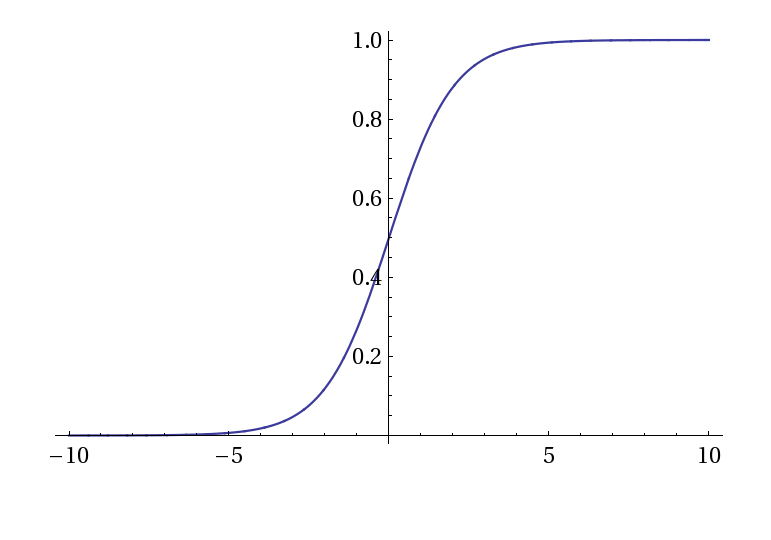
\includegraphics[width=.7\linewidth]{images/sigmoid.png}
  }
  \caption{Sigmoïde classique.}
  \label{fig:sigmoide1}
\end{figure}

\begin{figure}[ht]
  \centering
  \subcaptionbox{}[.7\linewidth][c]{
    $f(t) = \frac{1}{1 + e^{-0.02(t-350)}}$
  }
  \subcaptionbox{}[.7\linewidth][c]{
    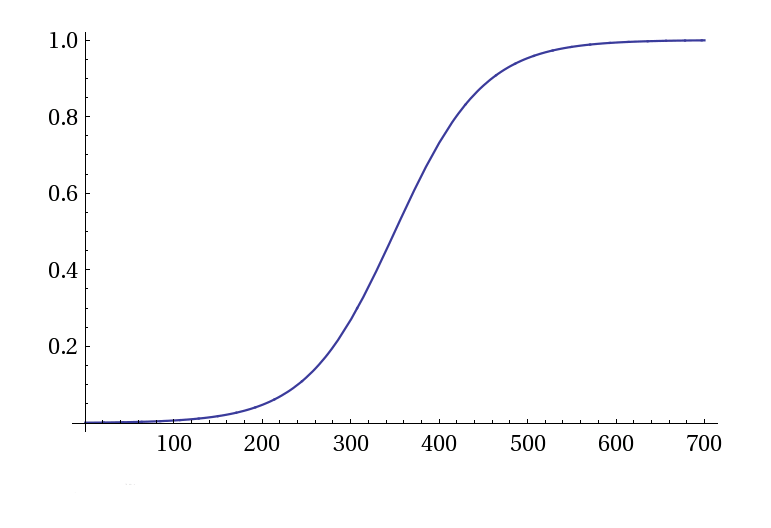
\includegraphics[width=.7\linewidth]{images/sigmoid-age.png}
  }
  \caption{Probabilité de changement d'état en fonction du temps.}
  \label{fig:sigmoide2}
\end{figure}

La figure \ref{fig:ac-stable} montre un automate cellulaire doté des
mêmes règles de transition et de la même configuration de départ mais
pour lequel l'âge des cellules est pris en compte.

\begin{figure}[h]
  \centering
  \subcaptionbox{$t = 0$}[.3\linewidth][c]{
    
\includegraphics[width=.3\linewidth]{images/sca_0.png}
  }
  \subcaptionbox{$t = 500$}[.3\linewidth][c]{
    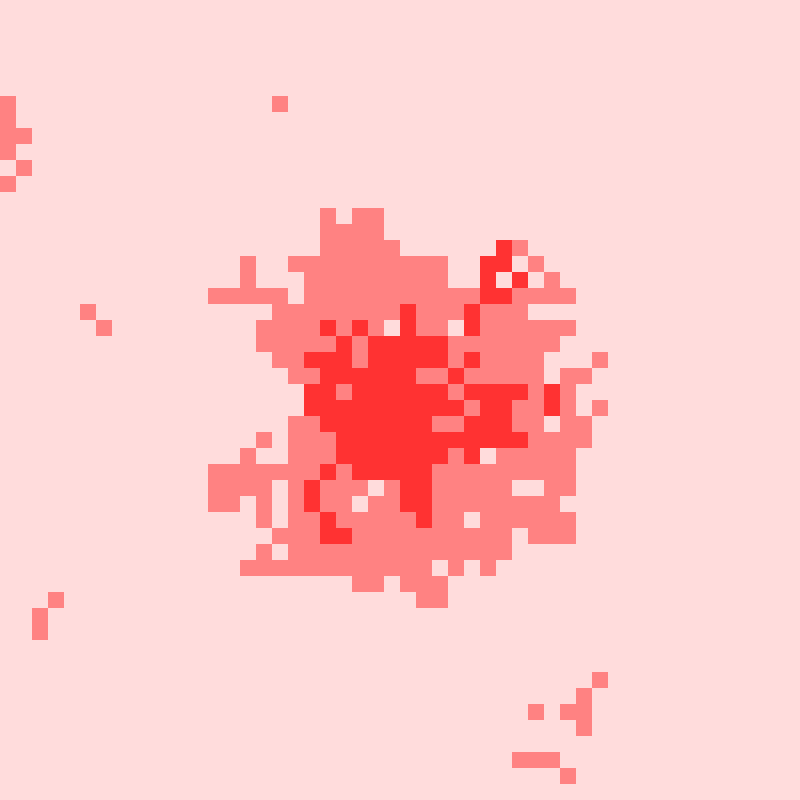
\includegraphics[width=.3\linewidth]{images/sca_500.png}
  }
  \subcaptionbox{$t = 1000$}[.3\linewidth][c]{
    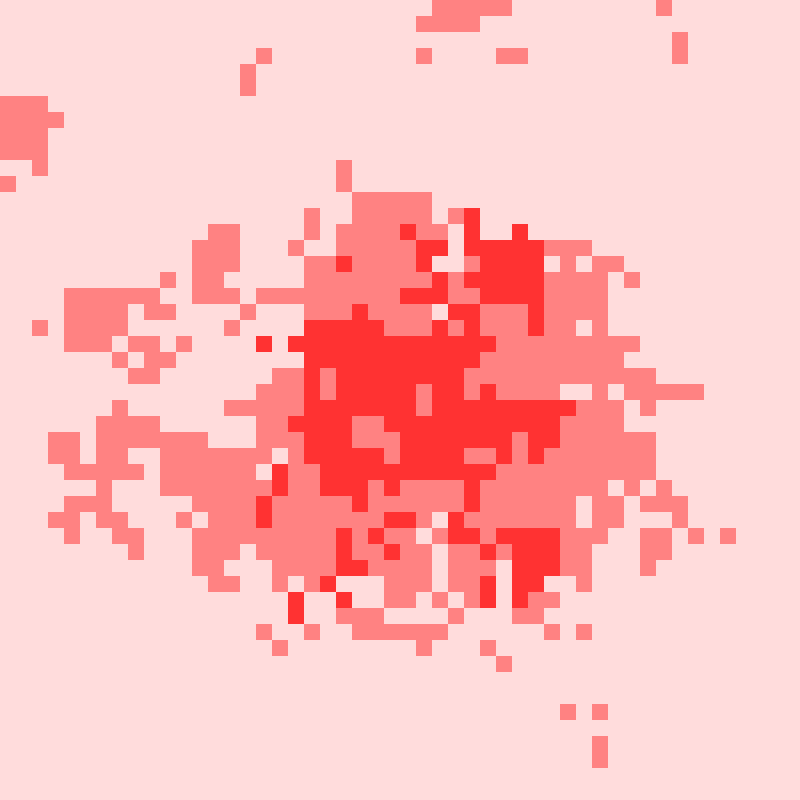
\includegraphics[width=.3\linewidth]{images/sca_1000.png}
  }

  \subcaptionbox{$t = 2000$}[.3\linewidth][c]{
    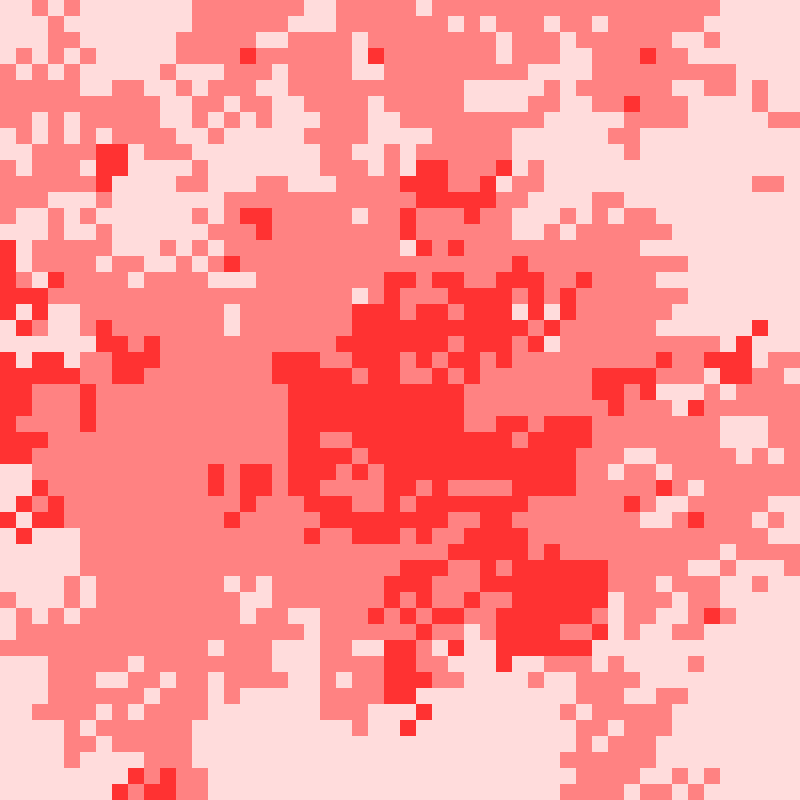
\includegraphics[width=.3\linewidth]{images/sca_2000.png}
  }
  \subcaptionbox{$t = 4000$}[.3\linewidth][c]{
    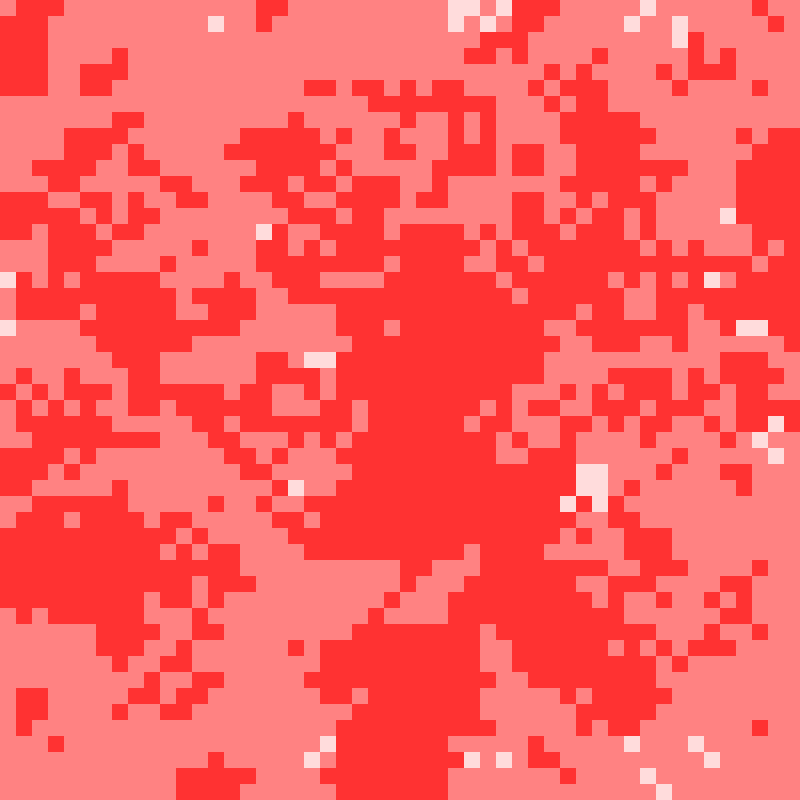
\includegraphics[width=.3\linewidth]{images/sca_4000.png}
  }
  \subcaptionbox{$t = 6000$}[.3\linewidth][c]{
    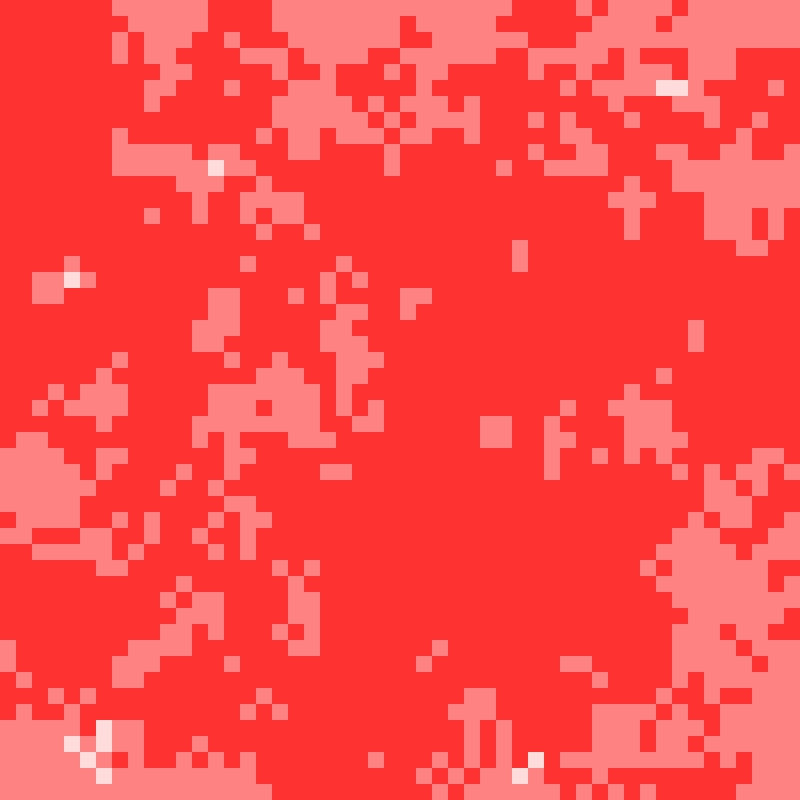
\includegraphics[width=.3\linewidth]{images/sca_6000.png}
  }
  \caption{Trois configurations successives de l'automate cellulaire
    stabilisé.}
  \label{fig:ac-stable}
\end{figure}

Les exemples précédents permettent d'illustrer les règles de
transition et met en évidence le problème de stabilité mais le
principe même de cet exposé est de se détacher de la régularité
spatiale contraignante des automates cellulaires et c'est à cet effet
que l'on a présenté le diagramme de Voronoï. À la manière des
automates cellulaires graphes de O'Sullivan \cite{O'Sullivan2000},
chaque parcelle verra son état varier en fonction de son
voisinage. Voisinage établit à partir de la topologie du diagramme de
Voronoï, lui-même issu des positions des centres des parcelles. Il est
à noter qu'à la différence de O'Sullivan, la couverture de l'espace
est totale puisque l'on ne représente pas les parcelles exactes mais
leur cellule de Voronoï et il est donc impossible que des zones vides
apparaissent entre les cellules.

Le \textit{graphe du bâti} prend ici la forme duale du diagramme de
Voronoï : la triangulation de Delaunay et décrit les relations de
voisinage. Un n\oe ud correspond au centre d'une parcelle et une arête
lie deux parcelles en tant que voisins.

\begin{figure}[h]
  \centering
  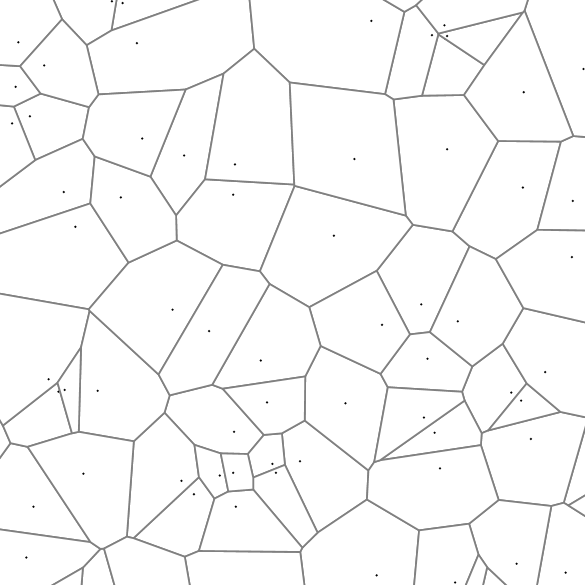
\includegraphics[width=.8\linewidth]{images/lots-graph.png}
  \caption{}
  \label{fig:lots-graph}
\end{figure}

APPLICATION DES REGLES

SIX IMAGES

La problématique étant d'étudier la coévolution de deux aspects
urbains, le viaire et le bâti, et non seulement l'évolution des
densités (qui ne sert que de support à l'essort de la ville), on a
préféré choisir une règle basique. il est néanmoins tout à fait
possible d'utiliser par la suite un automate cellulaire plus
sophistiqué pour améliorer le réalisme de la simulation.

\subsubsection{Placement des éléments potentiels}

Le second mécanisme place de nouvelles parcelles en bordure de la
ville et est responsable de sa croissance horizontale. Les nouvelles
parcelles placées bénéficient néanmoins d'un statut spécial car elles
sont considérées comme \textit{potentielles} et se démarquent des
parcelles \textit{construites} par leur impact sur l'évolution du
système :

\begin{itemize}
\item{L'état d'une parcelle potentielle dépend de toutes ses voisines}
\item{Une parcelle potentielle n'influence pas l'état des parcelles
  voisines construites}
\item{Une parcelle potentielle peut accueillir une route}
\end{itemize}

Cette influence unidirectionnelle dans le mécanisme cellulaire permet
à la parcelle potentielle d'être prête et accordée à son environnement
proche si elle est construite par la suite sans pour autant que les
parcelles déjà construites ne soient influencées par une parcelle
n'existant pas.

En quelques mots, le placement se déroule comme suit :

\begin{enumerate}
\item{On détermine les centres de la ville en fonction de la densité}
\item{On dépose sur un des centres une \textit{graine} mobile qui
  servira de générateur à la nouvelle parcelle}
\item{La graine se déplace sous l'influence des variables inhérentes à
  la ville}
\item{Quand la graine stoppe son mouvement, on y crée la parcelle}
\end{enumerate}

CENTRES?

Le déplacement de la graine est un processus pouvant potentiellement
prendre en compte de nombreuses variables. Dans l'application
d'exemple que l'on décrit, seules la densité et le placement des
routes peuvent guider la graine, car ce sont les seuls données
considérées. Cependant, on souhaite que le modèle soit extensible et
qu'il soit capable de supporter d'autres variables et contraintes : la
valeur des sols par exemple, ou bien la pente des zones envisagées ou
l'impossibilité de s'installer sur certains types de terrain (forêts,
plans d'eau). De cette idée de graine se déplaçant en fonction
d'influences diverses transpire un véritable aspect physique.

Pour rester en accord avec cet aspect physique on emploie un champ de
vecteur généré à partir de l'état du sytème urbain pour guider la
graine vers sa destination. Puisque de nombreux paramètres sont à
prendre en compte, on utilise un champ de vecteur par paramètre que
l'on souhaite exprimer puis on les combine, ce qui permet de pondérer
l'impact de chaque donnée.

Par exemple,

DENSITE

ROUTES

PATTERN

COMMENTAIRE

ARRET (AIRE ? SIGMOIDE ?)

\subsubsection{Construction des éléments potentiels}

ROUTES

PARCELLES

Le placement des parcelles se base sur le réseau routier puisque pour
qu'une parcelle soit construite, elle doit être reliée à au moins une
voie. Les voies sont quant à elle dépendantes des parcelles car selon
notre définition, une route est une arête de Voronoï d'une parcelle
(potentielle ou construite). Ce cycle est similaire à la morphogénèse
d'une ville car le processus d'extension que l'on observe dans un cas
d'urbanisme réel est le suivant :

\begin{enumerate}
\item{On prévoit d'installer des bâtiments en bordure de ville (les
  parcelles potentielles)}
\item{On construit une route avant de construire les parcelles}
\item{On construit plus tard les parcelles}
\end{enumerate}

DEJA DIT AILLEURS

les routes sont donc supports aux parcelles et leur construction est
motivée par la perspective de nouvelles parcelles. Les parcelles
potentielles étant placées par un mécanisme explicité plus haut, il
reste à sélectionner quelles arêtes du diagramme de Voronoï vont
devenir de véritables routes. On retrouve ici aussi le vocabulaire de
la potentialité utilisé au niveau parcellaire : les arêtes de Voronoï
sont considérées comme routes \textit{potentielles} et

La sélection les routes aptes à être construites doit être justifiée
par un besoin fonctionnel assurant une activité interne de la ville
efficace. Dans le cas du réseau viaire, on cherche donc à éviter les
engorgements et donc à organiser le maillage routier de façon à ce que
les zones à forte densité soient correctement desservies. DENSITE

NETWORK SIMPLEX

CONNEXITE

\section{Construction}

Notre système urbain est décrit sur deux niveaux; plus précisément,
par deux graphes. On distingue le graphe parcellaire du graphe viaire
car, bien qu'ils soient étroitement liés, ils représentent des couches
différentes du réseau urbain.

QQUAD MACHIN NON, 2 GRAPHES OUI

\subsection{Le graphe parcellaire}

Le graphe parcellaire correspond à la couche bâti. Ses n\oe uds sont
les centres des parcelles et chacune de ses arêtes représente une
relation de voisinage entre deux parcelles. Un diagramme de Voronoï
est nécessaire à la construction de ce graphe. Les seules données dont
l'on a besoin en entrée sont donc les positions centrales des
parcelles. Ces coordonnées peuvent être extraites de fichiers
d'informations géographiques mais dans un premier temps, et dans un
but llustratif, on se cantonne à utiliser des positions aléatoirement
choisies.

\begin{figure}
  \centering
  
\includegraphics[width=.6\linewidth]{images/logo-litis.png}
  \caption{}
  \label{fig:construction-bati1}
\end{figure}

La librairie Java JTS \cite{JTS} est spécialisée dans les traitements
géométriques et permet notamment de générer un diagramme de Voronoï à
partir d'une liste de points. Le résultat d'un tel traitement prend la
forme d'un ensemble de polygones, chacun représentant une cellule de
Voronoï, mais aucune autre information, notamment d'adjacence, n'est
fournie. Une fois le graphe parcellaire peuplé par des n\oe uds
positionnés aux coordonnées fournies plus tôt, il reste donc à
calculer les relations de voisinage et à ajouter les arêtes.

\begin{figure}
  \centering
  
\includegraphics[width=.6\linewidth]{images/logo-litis.png}
  \caption{}
  \label{fig:construction-bati2}
\end{figure}

Puisque l'on ne dispose que des polygones formant le diagramme de
Voronoï et des positions de leur centroïdes, on procède par
l'utilisation de tests géométriques. Naturellement, si deux cellules
sont en contact -- si elle partagent une arête -- alors on relie les
deux n\oe uds du graphe leur étant associés.

\begin{figure}
  \centering
  
\includegraphics[width=.6\linewidth]{images/logo-litis.png}
  \caption{}
  \label{fig:construction-bati3}
\end{figure}

La finalité de cet exercice n'est pas seulement de faire évoluer
l'automate cellulaire irrégulier que forme cette structure mais aussi
de lui permettre de se transformer au cours du temps, de s'étendre par
morphogenèse. INSERTION, DELETION

\subsection{Le graphe viaire}

Le graphe viaire correspond à la couche routière. Ses n\oe uds sont
des carrefours, aux croisements des parcelles, et ses arête des
voies. En pratique, pour différencier les routes potentielles des
routes construites, on attribue une étiquette spéciale à ces
dernières.

Comme lors de la construction du graphe parcellaire, on commence par
placer les n\oe uds (ici des carrefours) puis on veut les relier par
des arêtes (les routes).

Dans un premier temps, il nous faut déterminer les positions des
croisements qui feront office de n\oe uds dans le graphe viaire. Cette
phase est basée sur l'analyse du graphe parcellaire construit plus
tôt. Puisqu'une route entre deux bâtiments peut être définie par une
arête de Voronoï partagée entre deux parcelles, il est logique
d'admettre qu'un croisement correpond à un sommet de Voronoï partagée
par deux cellules ou plus. Le but de l'étape décrite est donc de
déterminer des groupes de cellules axées autour d'un même sommet
pivot.

\begin{figure}
  \centering
  
\includegraphics[width=.6\linewidth]{images/logo-litis.png}
  \caption{}
  \label{fig:construction-viaire1}
\end{figure}

On remarque que ces clusters de parcelles semblent être des
sous-graphes complets maximaux. Dans un premier temps, l'utilisation
de l'algorithme de Bron-Kerbosch a été envisagé (et appliqué,
inutilement !) mais certains cas particuliers nous laisse entrevoir
le fait qu'une contrainte supplémentaire est manquante. En effet, la
recherche d'une clique maximale par l'algorithme cité ne prend pas en
compte la nécessité que les cellules du cluster partagent un
sommet. Sur l'exemple de la figure ???, quatres cellules forment une
clique sans pour autant avoir un sommet de Voronoï en commun.

\begin{figure}
  \centering
  
\includegraphics[width=.6\linewidth]{images/logo-litis.png}
  \caption{}
  \label{fig:construction-viaire2}
\end{figure}

Puisque que l'algorithme de Bron-Kerbosch se révèle inadapté à l'usage
que l'on souhaitait en faire, il a été nécessaire de réflechir à une
autre méthode pour déterminer la position des carrefours et, surtout,
les parcelles à y associer. Une procédure a donc été mise en place
pour détecter ces clusters de parcelles pivotant autout d'un même
croisement. L'idée de base est de construire tous les groupes de
parcelles tels que :

\begin{itemize}
\item{Toutes les parcelles d'un groupe soient voisines entres elles}
\item{Les groupes soient maximaux}
\item{Les parcelles d'un groupe aient tous un sommet en commun}
\end{itemize}

Le dernier critère est la contrainte manquante à la définition des
cliques maximales. Concrètement, la construction de toutes ces listes
se résume à la construction de tous les cycles BLABLA. Ensuite,
ROUTES.

Un désavantage de cette méthode, outre sa complexité algorithmique,
est que seules les arêtes partagées par au moins deux parcelles
deviennent des routes. Ainsi, on remarque que les arête délimitant la
bordure de la ville (celles à l'extérieur du diagramme de Voronoï)
sont absentes. Il semble pourtant nécessaire que toutes les arête du
diagramme deviennent de potentielles voies car, dans notre modèle, la
route est le support du bâti. Et si aucune route ne peut se construire
à la bordure de la ville, aucun bâtiment ne s'y installera et la ville
ne grandira jamais.

Une solution MAIS

\begin{figure}
  \centering
  
\includegraphics[width=.6\linewidth]{images/logo-litis.png}
  \caption{}
  \label{fig:construction-viaire3}
\end{figure}

Finalement, nous nous sommes tournés vers une solution plus claire,
plus simple et permettant de transfomer en routes potentielles toutes
les arêtes sans exception : la construction puis la fusion de
sous-réseaux routiers. Dans le cadre de la tentative précédente,
chaque carrefour était identifié est placé dans le graphe viaire sous
la forme d'un n\oe ud mais la phase de placement des routes (la
liaison des n\oe uds par des arêtes) se faisaient une fois tous les
croisements placés. Il est clairement plus simple de créer pour chaque
parcelle un sous-réseau routier composé de ses propres sommets et de
els relier immédiatement. Une fois tous ces petits graphes crées ont
les fusionnent tous en prenant comme critère d'identification des
sommets leur position. On obtient au final un réseau routier complet
duquel aucune arête ne manque.

IMAGE

\section{Mesures}

HEUUUUUUUU...

DEGRE DES CARREFOURS

ELOIGNEMENT DE LA DENSITE PAR RAPPORT AU CENTRE GEOMETRIQUE

ELOIGNEMENT DE LA DENSITE PAR RAPPORT AUX CENTRES

TAILLE DES PARCELLES ? (BIAIS AU BORD)

\section{Conclusion}

RESUME

CONSTAT

PERSPECTIVES (DYNAMIQUES INTERNES, REALISME, INTERPRETATION, VRAIE VILLE)

\printbibliography

\end{document}
